

\documentclass[../../main.tex]{subfiles}



\begin{document}

\section{Amplificador}
Se construyó el amplificador de la figura \ref{fig:cir}. Tal como se observa en ella, el circuito es un colector común con una fuente de corriente, cuyo objetivo es polarizar y ser carga activa.

\begin{figure}[H]	
	\centering
	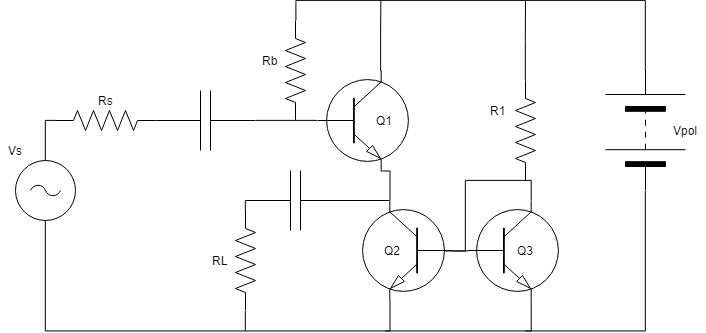
\includegraphics[width=0.7\textwidth]{imagenes/circuito.png}
	\caption{Amplificador}\label{fig:cir}
\end{figure}

Los valores de los compoenetes del circuito, son los indicados en la siguiente tabla
\begin{table}[h]
\begin{center}
\begin{tabular}{|l|l|}
\hline
Componente& Valor\\
\hline \hline
$R_s$ & $560 \Omega$  \\ \hline
$R_L$ & $2.2 K \Omega$  \\ \hline
$R_b$ & $680 K \Omega$  \\ \hline
$R_1$ & $10K\Omega$  \\ \hline
$C$ & $1uF$  \\ \hline
$V_{pol}$ & $20V$  \\ \hline
$Q_1 = Q_2 = Q_3$ & BC547  \\ \hline

\end{tabular}
\caption{Tabla de componentes} \label{tab:comp}
\end{center}
\end{table}


Las caracterisiticas de los transistores son las siguientes \footnote{Datasheet del BC547: Sparkfun.com. (2018). [online] Disponible en: https://www.sparkfun.com/datasheets/Components/BC546.pdf [Accedido 10 Nov. 2018].} :

\begin{table}[h]
\begin{center}
\begin{tabular}{|l|l|l|}
\hline
$hfe(DC)$& $hfe(AC)$&$V_A$\\
\hline \hline
110&165 &$98v$\\ \hline

\end{tabular}
\caption{Caracterisiticas de los transistores} \label{tab:qcar}
\end{center}
\end{table}

\subsection{Análisis del amplificador}
En esta sección se analizara la polarización y las características de pequeñas señales del amplificador.
\subsubsection{Polarización}
Para analizar la polarización del circuito, se pasivaran las fuentes del alterna. Lo primero a calcular es la fuente de corriente de la figura \ref{fig:ms}.

\begin{figure}[H]	
	\centering
	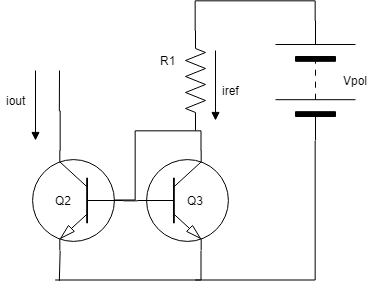
\includegraphics[width=0.4\textwidth]{imagenes/mirrorsource.png}
	\caption{Fuente de corriente constante}\label{fig:ms}
\end{figure}
Suponiendo que $Q_2$ y $Q_3$ son transistores iguales, tambien sus corrientes de base son iguales, por ende sus corriente de colector también lo son, y asumiendo que la corriente de base es despreciable frente a la de colector, entonces $I_{out}=I_{ref}$. 
\par Recorriendo la malla de entrada de $Q_3$ obtenemos que:
\begin{equation}
I_{ref}=\frac{V_{pol}-V_{be}}{R_1}\label{eq:mss}
\end{equation}

Conociendo las características de la fuente de corriente, se analizara la polarización del circuito:

\begin{figure}[H]	
	\centering
	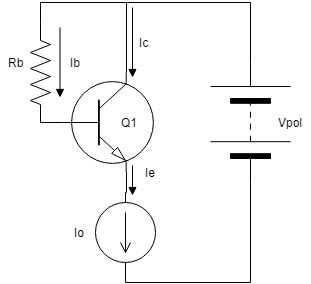
\includegraphics[width=0.4\textwidth]{imagenes/pol.png}
	\caption{Polarizacion del amplificador}
\end{figure}

Como$ I_e=I_o $ y $ I_o $ se obtiene a partir de la ecuación \ref{eq:mss}, entonces:
\begin{equation}
I_e=\left( hfe +1 \right)  Ib=I_o
\end{equation}
despejando $I_b$ se obtiene:
\begin{equation}
I_b=\frac{I_o}{hfe+1}
\end{equation}
\begin{equation}
I_{c}\cong I_o
\end{equation}

La tensión colector emisor se puede calculcar de la siguiente manera:
\begin{equation}
V_c=V_{pol}
\end{equation}
\begin{equation}
V_e=V_{pol} - R_b I_b - V_{be}
\end{equation}

restando ambas expresiones obtenemos,

\begin{equation}
V_{ce}=I_b R_b + V_{ce}
\end{equation}

Finalemnete reemplazando con los valores de los compoenentes, tabla \ref{tab:comp} y \ref{tab:qcar}, obtenemos :
$$I_b=17.5uA $$
$$I_c=1.93 mA $$
$$V_{ce}=12.6V $$


\end{document}
